\documentclass[UTF8]{article}
\usepackage{hyperref}
\usepackage{amsmath}%决策树
\usepackage{amsfonts}
\usepackage{cite}
\usepackage{natbib}
\newtheorem{theorem}{Theorem}
\newtheorem{lemma}{Lemma}
\newtheorem{proof}{Proof}[section]
\usepackage{graphicx}
\usepackage{subfigure}
%\usepackage{longtable}
\usepackage{algorithm}
\usepackage{algorithmic}
\usepackage{tikz}
\usetikzlibrary{shapes.geometric,fit,positioning,arrows,automata,calc}
\tikzset{
  main/.style={circle, minimum size = 5mm, thick, draw =black!80, node distance = 10mm},
  connect/.style={-latex, thick},
  box/.style={rectangle, draw=black!100}
}
%opening
\title{Universal Boost Decision Trees: A Unified Framework to Translate Optimization Methods into Boosting Algorithms}
\author{Zhang Jinxiong}

\begin{document}

\maketitle

\begin{abstract}

A  general paradigm is developed to translate  optimization methods to `boosting' algorithms. 
The gradient boost decision trees inspire  higher order boost decision trees.
And we translate the augmented Lagrangian methods to boosting algorithms with regularized cost fucntion.
The interaction of optimization methods and boosting algorithms is discussed in surrogate boosting decision trees.
It is first time to connent almost all optimization methods and boosting algorithms. 
It is why we call it as `universal boost'.
Although it is limited on boosted decision trees, the idea is easy to generalize to any boosting machine.
Results of several numerical tests are given which illustrate the theory.
\end{abstract}

\section{Introduction}
\href{https://web.stanford.edu/~hastie/Papers/AdditiveLogisticRegression/alr.pdf}{Jerome Friedman et al} assert that the Discrete AdaBoost algorithm (population version) builds
an additive logistic regression model via Newton-like updates for minimizing $E(e^{-yf(x)})$.
\href{https://users.soe.ucsc.edu/~manfred/pubs/C51.pdf}{Jyrki Kivinen, Manfred K. Warmuth},
\href{https://arxiv.org/pdf/0901.3590v1.pdf}{Chunhua Shen, Hanxi Li}
study some boosting algorithms from a entropy minimization perspective.
The gradient boost machine algorithms seems far from continuous optimization methods.
%http://parnec.nuaa.edu.cn/seminar/2013_Spring/20130416/slides-NJU-CS.pdf
\href{http://docs.salford-systems.com/GreedyFuncApproxSS.pdf}{Gradient boost machine} is usually considered as functional gradient descent.
There are many \emph{gradient-like boosting machines} to fit the profitable directions different from negative gradients
such as 
\href{https://papers.nips.cc/paper/1766-boosting-algorithms-as-gradient-descent.pdf}{AnyBoost},
\href{https://arxiv.org/pdf/1510.02558.pdf}{Functional Frank-Wolfe Boosting},
\href{https://arxiv.org/abs/1603.02754}{XGBoost},
\href{https://easychair.org/publications/open/pCtK}{Historical Gradient Boost Machine},
\href{https://arxiv.org/abs/1803.02042}{Accelerated Gradient Boosting},
\href{https://arxiv.org/abs/1903.08708}{Accelerating Gradient Boosting Machine},
\href{https://arxiv.org/abs/1910.03225}{NGBoost}.

It seems that optimization methods can be mapped to boosting algorithms.
However, it is not clear how to translate continuous optimization methods to their functional version such as ADMM.
We will show that there is a unified framework to translate each optimization method to boosting algorithm. 
\section{Gradient Boost Decision Trees}

Boosted decision tree or multiple additive regression tree is the sum of successive decision tree
$$F(x)=\sum_{n=1}^{T}f_{t}(x)$$
where $f_{n}$ relies on the outputs of its `parent tree' $f_{n-1}$ for $n=2, 3,\cdots, N$.

The following algorithm describe the  gradient boost decision  as  boosted decision trees

\begin{algorithm}[h]
\caption{Gradient Boost Decision Trees}
\begin{algorithmic}[1]
\STATE {Input training data set $\{(x_n, y_n)\mid x_n\in\mathrm{X}\subset\mathbb{R}^{p}, y_n\in\mathbb R,n=1,2,\cdots, N\}$}
\STATE{ Initialize $f_0=\arg\min_{\gamma}\sum_{i=1}^{N}L(x_i, \gamma)$}
\FOR{$t = 1, 2, \dots, T$}
\FOR{$i = 1, 2,\dots , N$}
\STATE Compute $r_{i,t}=-{[\frac{\partial L(\mathrm{y}_i, f(x_i))}{\partial f(x_i)}\mid_{f=F^{(t-1)}}]}.$
\ENDFOR
\STATE  Fit a regression tree to the targets $r_{i,t}$   giving terminal regions
   $$R_{j,m}, j = 1, 2,\dots , J_m. $$
%\label{code: TrainBase:getc}
\FOR{$j = 1, 2,\dots , J_m$ }
\STATE  Compute $\gamma_{j,t}=\arg\min_{\gamma}\sum_{x_i\in R_{j,m}}{L(\mathrm{y}_i, F^{(t-1)}(x_i)+\gamma)}$.
\ENDFOR
\STATE  $f_t={\sum}_{j=1}^{J_m}{\gamma}_{j, t} \mathbb{I}(x\in R_{j, m})$
\STATE Update $F^{(t)} = F^{(t-1)}+\nu f_t,\nu\in(0, 1)$
\ENDFOR
\STATE Output $F^{(T)}$.
\end{algorithmic}
\end{algorithm}
%版权声明:本文为CSDN博主「xmjdh」的原创文章,遵循 CC 4.0 BY-SA 版权协议,转载请附上原文出处链接及本声明。
%原文链接:https://blog.csdn.net/lqhbupt/article/details/8723478

%For example, \href{https://stanfordmlgroup.github.io/projects/ngboost/}{NGBoost} has three abstract modular components as following
%
%\includegraphics[scale=0.4]{blocks.png}
%
%where the natural gradient as feedback signal is uased to train another base learner.

In gradient boost decision tree, it takes additive training:
$$\gamma_{j,t}=\arg\min_{\gamma}\sum_{x_i\in R_{j,m}}L(\mathrm{y}_i, \underbrace{F^{(t-1)}(x_i)+\gamma}_{\text{additive training}})$$
which results as weighted sum of decision trees.
Here $\gamma_{j, t}$ is expected to be parallel of $-{[\frac{\partial L(\mathrm{y}_i, f(x_i))}{\partial f(x_i)}\mid_{f=F^{(t-1)}}]}= -g_{t-1, i}$
thus $F^{(t)}(x_i)\approx F^{t-1}(x_i)-\alpha g_{t-1, i}$.
%The following inequality holds for some $\alpha\in(0,1)$ if the loss function $L$ is smooth
%$$\sum_{i=1}^{N}L(\mathrm{y}_i, F^{(t-1)}(x_i))\geq \sum_{i=1}^{N}{L(\mathrm{y}_i, F^{(t-1)}(x_i)-\alpha[\frac{\partial L(\mathrm{y}_i, f(x_i))}{\partial f(x_i)}\mid_{f=F^{(t-1)}}]).$$

If let $F^{(t-1)}(x_i)=\tilde{y}_i$, the following inequality holds for some $\alpha\in(0,1)$ if the loss function $L$ is smooth

$$\sum_{i=1}^{N} L(\mathrm{y}_i, \tilde{y}_i)\geq \sum_{i=1}^{N} L(\mathrm{y}_i, \tilde{y}_i-\alpha [\frac{\partial L(\mathrm{y}_i,\tilde{y}_i)}{\partial \tilde{y}_i}]).$$
This is basic idea of gradient descent.
%We will revisit the connection of optimization and boosting based on the
%\href{https://papers.nips.cc/paper/1766-boosting-algorithms-as-gradient-descent.pdf}{AnyBoost} and
%\href{https://web.stanford.edu/~hastie/Papers/buehlmann.pdf}{BOOSTING ALGORITHMS: REGULARIZATION, PREDICTION AND MODEL FITTING}.
And the gradient descent is updated by
$$\theta^{(t+1)}=\theta^{(t)}-\alpha_t\nabla_{\theta}L(\theta^{(t)})$$
for  $t=0,1,2,\cdots, T-1$.
The final result of gradient descent is
$$\theta^{(T)}=\theta^{(0)}-\sum_{t=1}^{T-1}\alpha_t\nabla_{\theta}L(\theta^{(t)}).$$
If we replace the $\theta^{(T)}(\theta^{(0)})$ with the gradient boost decision trees $F^{(T)}(f_0)$ 
and $-\nabla_{\theta}L(\theta^{(t)})$  with the decision tree $f_t$ for $t=1,2,\cdots,T-1$, 
we will obtain
$$F^{(T)}=f_0+\sum_{t=1}^{T-1}\alpha_t f_t.$$
In gradient boost decision trees, a tree $f_t$ is used to fit the negative gradient $-\frac{\partial L(\mathrm{y}_i,\tilde{y}_i)}{\partial \tilde{y}_i}$ for $i=1,2,\cdots, N$ so that it brings some noise or error in this step.
So we say that it is analogous to gradient descent.

In optimization, we call the point $\gamma$ at point $\tilde{y}_i$ as profitable direction if
$$\sum_{i=1}^{N} L(\mathrm{y}_i, \tilde{y}_i)\geq \sum_{i=1}^{N} L(\mathrm{y}_i, \tilde{y}_i+\gamma).$$
There are many \emph{gradient-like boosting machines} to fit the descent directions different from negative gradients
such as \href{https://arxiv.org/pdf/1510.02558.pdf}{Functional Frank-Wolfe Boosting},
\href{http://www.svcl.ucsd.edu/publications/conference/2011/TaylorBoost.pdf}{TaylorBoost},
\href{https://arxiv.org/abs/1603.02754}{XGBoost},
\href{https://arxiv.org/abs/1910.03225}{NGBoost}.
It is also the basic idea behind \href{https://papers.nips.cc/paper/1766-boosting-algorithms-as-gradient-descent.pdf}{AnyBoost}.

What is more,
\href{https://easychair.org/publications/open/pCtK}{Historical Gradient Boost Machine},
\href{https://arxiv.org/abs/1803.02042}{Accelerated Gradient Boosting},
\href{https://arxiv.org/abs/1903.08708}{Accelerating Gradient Boosting Machine} extend the gradient boost methods to momentum boost methods.
\href{https://arxiv.org/abs/1603.02754}{XGBoost} extend the gradient boost methods to second order boost methods.
Any techniques in gradient-based optimization methods can be applied to
gradient boost decision trees such as the distributed optimization techniques,
acceleration techniques, variance reduction techniques.
%It is really a bridge between continuous optimization methods
%and booted decision tree algorithms by replacing the targets with update formula
%in optimization methods.

Note that the following relation always holds for most loss function:
$$\ell(\mathrm{y}_i, f(x_i))=0\iff \mathrm{y}_i = f(x_i)\iff \frac{\partial \ell(\mathrm{y}_i, f(x_i))}{\partial f(x_i)}\mid_{f=F^{(t-1)}}=0$$
which means if $f(x_i)=\mathrm{y}_i$ the value $0$ will be learnt in next decision tree.
In another words, the gradient is always to be $0$  when the loss is $0$.
And the outputs is a constant in vanilla decision tree for different input in the same leaf
so that the new targets $r_{i,t}$ and $r_{j, t}$ are equal if $x_i, x_j$ are output in the same leaf and $y_i=y_j$.
As a result, such pair $x_i, x_j$ tends to be in the same terminal region in the next tree.
The samples in the same terminal region with different targets tend to be seperated in the next tree.
The gradients is used to build the next decision tree.

``If I have seen further, it is by standing on the shoulders of giants."
The new targets $\{f_{t-1}(x_i)-\alpha_{i,t}g_{i,t}\}$ are the shoulders of giants in decision tree for $i=1,2,\cdots, N, t=1,2,\cdots, T$.
In next section, we will translate higher order optimization methods to boosting algorithms.

\section{Higher Order Boost Decision Trees}

\href{https://arxiv.org/abs/1603.02754}{XGBoost} extends the gradient boost to the second order boost method.
We can generalize much higher order boost decision tree.
Even gradient is computed in xGBoost, it is univariate rather than multivariate so that quasi-Newton methods cannot play a role in our framework. 

Halley's method is a third order method to find the roots of nonlinear equations.
At point $X_n$, the next point $X_{n+1}$ in Halley's method is found by :
\begin{equation}
X_{n+1}=X_n-\frac{2f(X_n)f^{\prime}(X_n)}{2[f^{\prime}(X_n)]^2 - f(X_n)f^{\prime\prime}(X_n)}.\label{Halley's Method}
\end{equation}
\href{https://ms.yccd.edu/Data/Sites/1/userfiles/facstaff/jthoo/cvandpubs/papers/halley.pdf}{It} is proved to be cubical convergence insofar as the number of significant digits eventually triples with each iteration.
See some examples of \href{https://observablehq.com/@herbps10/halleys-method}{Halley's method} visualized by \href{https://observablehq.com/@herbps10}{Herb Susmann}.

Now we apply Halley's method to the equation $g(x)=0$:
\begin{equation}
x_{n+1}=x_n-\frac{2g(x_n)g^{\prime}(x_n)}{2[g^{\prime}(x_n)]^2 - g(x_n)g^{\prime\prime}(x_n)}
\end{equation} 
where $g(x)=\frac{\partial L(\mathrm{y}, f(x))}{\partial f(x)}$, i.e., $g(x)$ is the derivative function of the ouput of $x$. It is a fixed point iteration to find the minimal values of $L(\mathrm{y}, f(x))$.

Then we translate the Halley's method to a third order boosting algorithm.
%\href{https://archive.lib.msu.edu/crcmath/math/math/h/h030.htm}{Halley's Method}
%\href{https://ijpam.eu/contents/2016-111-1/6/6.pdf}{modefied Helley's method}
%http://www.optimization-online.org/DB_FILE/2007/03/1610.pdf
%https://observablehq.com/@herbps10/halleys-method
%The rate of convergence in terms of the function value for 
%\href{https://ideas.repec.org/p/cor/louvco/2018005.html}{the accelerated third-order scheme}
%reaches the level $O(1/k^4)$, where $k$ is the number of iterations. 
%It is expected to have better performance of higher order  boost decision trees,
%i.e., to reduce the communication cost.

\begin{algorithm}[h]
  \caption{Third Order Boost Decision Trees}
  \begin{algorithmic}[1]
  \STATE {Input training data set $\{(x_n, y_n)\mid x_n\in\mathrm{X}\subset\mathbb{R}^{p}, y_n\in\mathbb R,n=1,2,\cdots, N\}$}
  \STATE{ Initialize $f_0=\arg\min_{\gamma}\sum_{i=1}^{N}L(x_i, \gamma)$}
  \FOR{$t = 1, 2, \dots, T$}
  \FOR{$i = 1, 2, \dots, N$}
  \STATE Compute $r_{i,t}=T_t(x_i)$
  \ENDFOR
  \STATE  Fit a regression tree to the targets $r_{i,t}$   giving terminal regions
     $$R_{j,m}, j = 1, 2,\dots , J_m. $$
  \label{code: TrainBase:getc}
  \FOR{$j = 1, 2,\dots , J_m$ }
  \STATE  Compute $\gamma_{j,t}=\arg\min_{\gamma}\sum_{x_i\in R_{j,m}}{L(\mathrm{y}_i, F^{(t-1)}(x_i)+\gamma)}$.
  \ENDFOR
  \STATE  $f_t={\sum}_{j=1}^{J_m}{\gamma}_{j, t} \mathbb{I}(x\in R_{j, m})$.
  \STATE Update $F^{(t)} = F^{(t-1)}+ f_t$.
  \ENDFOR
  \STATE Output $F^{(T)}$.
  \end{algorithmic}
\end{algorithm}
Here $T_t(x_i)=-\frac{2g_t(x_i)g_t^{\prime}(x_i)}{2[g_t^{\prime}(x_i)]^2 - g_t(x_i)g_t^{\prime\prime}(x_i)}$ and
$g_t(x_i)=\frac{\partial L(\mathrm{y}_i, f(x_i))}{\partial f(x_i)}\mid_{f=F^{(t-1)}}$,
$g_t^{\prime}(x_i)=\frac{\mathrm d g_t(x_i)}{\mathrm d  f(x_i)}\mid_{f=F^{(t-1)}}$,
$g_t^{\prime\prime}(x_i)=\frac{\mathrm d g_t^{\prime}(x_i)}{\mathrm d  f(x_i)}\mid_{f=F^{(t-1)}}$.
Note that it works only when $2[g_t^{\prime}(x_i)]^2 - g_t(x_i)g_t^{\prime\prime}(x_i)\not=0$. And when $g(x)=0\quad\forall x\in\mathbb{R}$, it finds a fixed point.
When $g_t^{\prime\prime}(x_i)=0$, it is exactly the Newton's method.
All the technoques used in xGBoost can apply to this third order boost decision trees.
So that it is a direct extension of xGBoost.

%https://sites.google.com/site/optneurips19/
% https://jasondlee88.github.io/
% https://higher.readthedocs.io/en/latest/
% https://bbullins.github.io/
% https://qubovert.readthedocs.io/en/latest/BO/HOBO.html
%\href{https://alfresco.uclouvain.be/alfresco/service/guest/streamDownload/workspace/SpacesStore/aabc2323-0bc1-40d4-9653-1c29971e7bd8/coredp2018_05web.pdf?guest=true}{Implementable tensor methods in unconstrained convex optimization}
Higher order optimzizatin methods include \href{https://dl.acm.org/citation.cfm?id=2643338}{Cauchy’s method}.
%https://core.ac.uk/download/pdf/82046338.pdf
\section{Surrogate Boost Decision Trees}

%The surrogate principle in continuous optimization palys a lead role in finding new targets $r_{i,t}$.
The surrogate principle is to optimze a simple surrogate objective function  at each iteration 
instead of the original complex objective function.
%https://www.sciencesmaths-paris.fr/upload/Contenu/HM%202014/schoenauer.pdf
For example, our aim is to solve an optimization problem of the following form
\begin{equation}\label{eq:fw_objective}
  \arg\min_{\boldsymbol{x} \in \mathcal{X}} f(\boldsymbol{x}).
\end{equation}
Given initial estimates $\boldsymbol{x}_0$ and surrogate objective function $Q(x_t, x)$,
it is updated via 
$$\boldsymbol{x}_{t+1}=\arg\min_{x}Q_t(x),$$
and it is usually $f(\boldsymbol{x}_{t+1})\leq f(\boldsymbol{x}_t)$.
Generally, it is required that $\lim_{t\to\infty}{x}_{t}=x^{\star}\in \arg\min_{\boldsymbol{x} \in \mathcal{X}} f(\boldsymbol{x})$.
The surrogate objective function $Q(x_t, x)$ is usually simpler to optimze than original function
$f(\boldsymbol{x})$.

\begin{algorithm}[h]
  \caption{Surrogate Boost Decision Trees}
  \begin{algorithmic}[1]
  \STATE {Input training data set $\{(x_n, y_n)\mid x_n\in\mathrm{X}\subset\mathbb{R}^{p}, y_n\in\mathbb R,n=1,2,\cdots, N\}$}
  \STATE{ Initialize $f_0=\arg\min_{\gamma}\sum_{i=1}^{N}L(x_i, \gamma)$}
  \FOR{$t = 1, 2, \dots, T$}
  \FOR{$i = 1, 2, \dots , N$}
  \STATE Compute $r_{i,t}=\arg\min_{x}Q_t(y_i,F^{(t-1)}(x_i)+x)$.
  \ENDFOR
  \STATE  Fit a regression tree to the targets $r_{i,t}$ giving terminal regions
     $$R_{j,m}, j = 1, 2,\dots , J_m. $$
  \FOR{$j = 1, 2,\dots , J_m$ }
  \STATE Compute $\gamma_{j,t}=\arg\min_{\gamma}\sum_{x_i\in R_{j,m}}{L(\mathrm{y}_i, F^{(t-1)}(x_i)+\gamma)}$.
  \ENDFOR
  \STATE $f_t={\sum}_{j=1}^{J_m}{\gamma}_{j, t} \mathbb{I}(x\in R_{j, m})$.
  \STATE Update $F^{(t)} = F^{(t-1)}+f_t$.
  \ENDFOR
  \STATE Output $F^{(T)}$.
  \end{algorithmic}
\end{algorithm}

In this framework, we can extend  `expectation maximization' type boosting algorithms for probabilistic predictiona as 
\href{https://arxiv.org/abs/1910.03225}{NGBoost}.

The surrogate minimization principle is applied to boosting algorithms.
We are closer to the ultimate goal: translate the optimziation methods to boosting algorithms.

%\href{http://fa.bianp.net/teaching/2018/eecs227at/surrogate.html}{A unifying principle: surrogate minimization}
%\href{https://arxiv.org/pdf/1402.4419.pdf}{INCREMENTAL MAJORIZATION-MINIMIZATION OPTIMIZATION}

\section{ADMM Boost Decision Trees}

Now  we take alternating direction method of multipliers (ADMM) into consideration.

ADMM is aimed to solve the following convex optimization problem:
\begin{equation}
\min F(x,y) \{=f(x)+g(y)\}  \\
        \text{  subject to }\quad  Ax+By =b, x\in\mathbf{X}, y\in\mathbf{Y},\label{ADMM}
\end{equation}
where $f(x),g(y), \mathbf{X, Y}$ are convex; ${A}$ and ${B}$ are matrices.
Its augmented Lagrangian is defined as $L_{\beta}(x, y)=f(x)+g(y) - \lambda^{T}(Ax + By -b)+ \frac{\beta}{2}{\|Ax + By - b\|}_{2}^{2}$.
ADMM at step $t$ is described as following:
\begin{enumerate}
\item $x^{k+1}=\arg\min_{x\in\mathbf{X}}L_{\beta}(x,y^{\color{blue}{k}},\lambda^{\color{blue}{k}});$
\item $y^{k+1}=\arg\min_{y\in\mathbf{Y}} L_{\beta}(x^{\color{red}{k+1}}, y, \lambda^{\color{blue}{k}});$
\item $\lambda^{k+1} = \lambda^{k} - \beta (Ax^{\color{red}{k+1}} + By^{\color{red}{k+1}}-b).$
\end{enumerate}

%Here $L_{\beta}(x, y)=f(x)+g(y) - \lambda^{T}(Ax + By -b)+ \frac{\beta}{2}{\|Ax + By - b\|}_{2}^{2}$.

The  aim boosting algorithms is to find a decision tree $f^{\star}$ to minimize the following function
 $$\arg\min_{f}\sum_{i=1}^{N}\ell(y_i, f(x_i))+r\sum_{i=1}^{N}|f(x_i)| \text{  subject to $z_i=f(x_i)$}$$
where $\ell(y_i, f(x_i))$ is the loss of sample $(x_i, y_i)$ and $r\sum_{i=1}^{N}|f(x_i)|$ is the regularization term.
Note that the loss function $\ell(\cdot, \cdot)$ is usually convex and $f$ is a decision tree (region-wise linear function), so the above cost function is convex.
\begin{algorithm}[h]
  \caption{ADMM Boost Decision Trees}
  \begin{algorithmic}[1]
  \STATE {Input training data set $\{(x_n, y_n)\mid x_n\in\mathrm{X}\subset\mathbb{R}^{p}, y_n\in\mathbb R,n=1,2,\cdots, N\}$}
 % \label{code:recentStart}
  \STATE {Initialize $f_0=\arg\min_{\gamma}\sum_{i=1}^{N}L(x_i, \gamma)$}
  \FOR{$t = 1, 2, \dots, T$}
  \FOR{$i = 1, 2,\dots , N$}
  %\STATE  compute  $a_{i,t}=\arg\min_{\gamma_i}L_{\beta}^{(t)}(\gamma_i, z, \lambda)$
  %\STATE  compute new targets $r_{i,t}=a_{i,t}+f_t(x_i)$
  \STATE  Compute $r_{i,t}=\arg\min_{\gamma_i}L_{\beta}^{(t)}(\gamma_i, z_i, \lambda_i)$.
  \ENDFOR
  \STATE  Fit a regression tree to the targets $r_{i,t}$ giving terminal regions
     $$R_{j,m}, j = 1, 2,\dots , J_m. $$
  %\label{code:TrainBase:getc}
  \FOR{$j = 1, 2,\dots , J_m$ }
  \STATE  Compute $\gamma_{j, t}=\arg\min_{\gamma}\sum_{x_i\in R_{j,m}}{L(\mathrm{y}_i, \gamma)}$.
  \ENDFOR
  \STATE $f_t={\sum}_{j=1}^{J_m}{\gamma}_{j, t} \mathbb{I}(x\in R_{j, m})$.
  \STATE Update $F^{(t)} = F^{(t-1)}+f_t$.
  \ENDFOR
  \STATE  Compute $z^{t+1}=\arg\min_{z} \sum_{i=1}^{N}L_{\beta}^{(t)}(r_{i,t},z_i,\lambda^{t}_i)$.
  \STATE  Compute $\lambda^{t+1}=\arg\min_{\lambda}\sum_{i=1}^{N} L_{\beta}^{(t)}(r_{i,t},z^{t+1}_i,\lambda_i)$
  %\label{code:TrainBase:pos}
  \STATE  Output $F^{(T)}$.
  %\label{code:recentEnd}
  \end{algorithmic}
\end{algorithm}

Here the augmented Lagragian is given by

\begin{align}
L_{\beta}^{(t)}(\gamma_i, z_i, \lambda_i) \nonumber
& =\ell(y_i, f_{t-1}(x_i) + \gamma_i) \\ \nonumber
&+ r {|z_i|}_1 -\left<z_i-(f_{t-1}(x_i) + \gamma_i),\lambda_i\right>\\ \nonumber
&+ \frac{\beta}{2}{|z_i-(f_{t-1}(x_i) + \gamma_i)|}. \nonumber
\end{align}

And $f(\cdot)$ is a decision tree; $\ell(\cdot, \cdot)$ is the loss function.
%https://statweb.stanford.edu/~candes/math301/Lectures/Consensus.pdf

This scheme is more suitable for the regularized cost function.
In general, all the optimization methods for the optimizaion problem \ref{ADMM} can be tranlated to 
boosting algorithms.
It is the first time to translate the augmented Lagragian method to boosting algorithms.
And this framework can be generalized to any operator splitting optimization method.

\section{Accelerating Boosting}

It may not be intuitive but it is true that all the optimization methods associated with the  above boosting algorithms are fixed point iteration.
For example, the surrogate optimization is given by
$$x_{i+1}=\arg\min_{x}Q(x_i, x)$$
so that a fixed point satisfies $x_{i}=\arg\min_{x}Q(x_i, x)$. 
ADMM is a Gaussian-Seidel type fixed point iteration.

We combine gradient boosting and  accelerated gradient methods to design new algorithms such as
\href{https://easychair.org/publications/open/pCtK}{Historical Gradient Boost Machine},
\href{https://arxiv.org/abs/1803.02042}{Accelerated Gradient Boosting},
\href{https://arxiv.org/abs/1808.09670}{Accelerated proximal boosting},
\href{https://arxiv.org/abs/1903.08708}{Accelerating Gradient Boosting Machine}.
% https://github.com/lrouviere/AGB

\href{https://dash.harvard.edu/bitstream/handle/1/34773632/Extrapolation%20Algorithm%20w%20Appendix.pdf}{Anderson Acceleration}
is a generic technique for accelerating the convergence of the fixed point iteration in the applied mathematics community.  
And it is alos called as  Anderson Mixing in the computational quantum mechanics community.
 

We want to verify that if Anderson acceleration (AA) can improve the convergence rate of 
boosting algorithms based on general fixed point iterations.


\begin{algorithm}[h]
  \caption{Accelerating Surrogate Boost Decision Trees}
  \begin{algorithmic}[1]
  \STATE {Input training data set $\{(x_n, y_n)\mid x_n\in\mathrm{X}\subset\mathbb{R}^{p}, y_n\in\mathbb R,n=1,2,\cdots, N\}$, $m$}
  \STATE{ Initialize $f_0=\arg\min_{\gamma}\sum_{i=1}^{N}L(x_i, \gamma)$}
  \FOR{$t = 1, 2, \dots, T$}
  \FOR{$i = 1, 2, \dots , N$}
  \STATE Compute $\tilde{r}_{i,t}=\arg\min_{x}Q(f_t(x_i), F^{(t-1)}(x_i)+x)$.
  \STATE {Compute $\alpha^{\star}=\arg\min_{\alpha}\|\alpha_t\tilde{r}_{i,t}+\alpha_{t-1}\tilde{r}_{i,t-1}, \cdots+\alpha_{t-m}\tilde{r}_{i,t-m}\|_2^2$ subject to $\sum_{i=t-m}^{t}\alpha_i=1$.}
  \STATE Compute $r_{i,t}^{\star}=\left<\alpha^{\star}, \tilde r_i\right>=\sum_{n=t-m}^{t}\alpha_n^{\star}\tilde{r}_{i,n}$
  \ENDFOR
  \STATE  Fit a regression tree to the targets $r_{i,t}^{\star}$ giving terminal regions
     $$R_{j,m}, j = 1, 2,\dots , J_m. $$
  \FOR{$j = 1, 2,\dots , J_m$ }
  \STATE Compute $\gamma_{j,t}=\arg\min_{\gamma}\sum_{x_i\in R_{j,m}}{L(\mathrm{y}_i, F^{(t-1)}(x_i)+\gamma)}$.
  \ENDFOR
  \STATE $f_t={\sum}_{j=1}^{J_m}{\gamma}_{j, t} \mathbb{I}(x\in R_{j, m})$.
  \STATE Update $F^{(t)} = F^{(t-1)}+f_t$.
  \ENDFOR
  \STATE Output $F^{(T)}$.
  \end{algorithmic}
\end{algorithm}

% https://arxiv.org/pdf/1810.08455.pdf
% https://www.csm.ornl.gov/workshops/applmath11/documents/Walker_LinearAlgebra.pdf
% https://epubs.siam.org/doi/abs/10.1137/10078356X
% https://web.wpi.edu/Pubs/ETD/Available/etd-112409-140359/unrestricted/pni.pdf
% https://arxiv.org/abs/1909.00470
% https://ieeexplore.ieee.org/document/8461063

\section{Stochastic Boosting}

\href{http://web.mit.edu/haihao/www/papers/RGBM.pdf}{Randomized Gradient Boosting Machine}
\href{http://docs.salford-systems.com/StochasticBoostingSS.pdf}{Stochatsic Gradient Boost Machine}

\section{Theoretical Analyses}

We translate the optimization methods to  boosting algorithms in the syntax of iterative form.
We only focus on the syntax in the above section.
In this section, we will focus on the semantics.
We want to answer if this translation preserve the complexity or converegnce speeed in some sense. 

\subsection{Rademacher Complexity Bound}

\href{https://arxiv.org/pdf/1510.02558.pdf}{Functional Frank-Wolfe Boosting}

\subsection{Convergence Analysis}

\href{https://arxiv.org/pdf/1903.08708.pdf}{Accelerating Gradient Boosting Machine}
\href{http://web.mit.edu/haihao/www/papers/RGBM.pdf}{Randomized Gradient Boosting Machine}

\subsection{Generalization Analysis}

\href{https://jeremykun.com/2014/01/02/probably-approximately-correct-a-formal-theory-of-learning/}{Probably Approximately Correct Learning}

\href{http://students.cse.tamu.edu/xingwang/courses/ece689607/regret_boost.pdf}{”A decision-theoretic generalization of on-line learning and an application to boosting}

https://arxiv.org/pdf/0804.2752.pdf

\section{Experiments}

Evaluation of these algorithms is elaborate.

  \includegraphics[scale=0.5]{GBDT.png}
  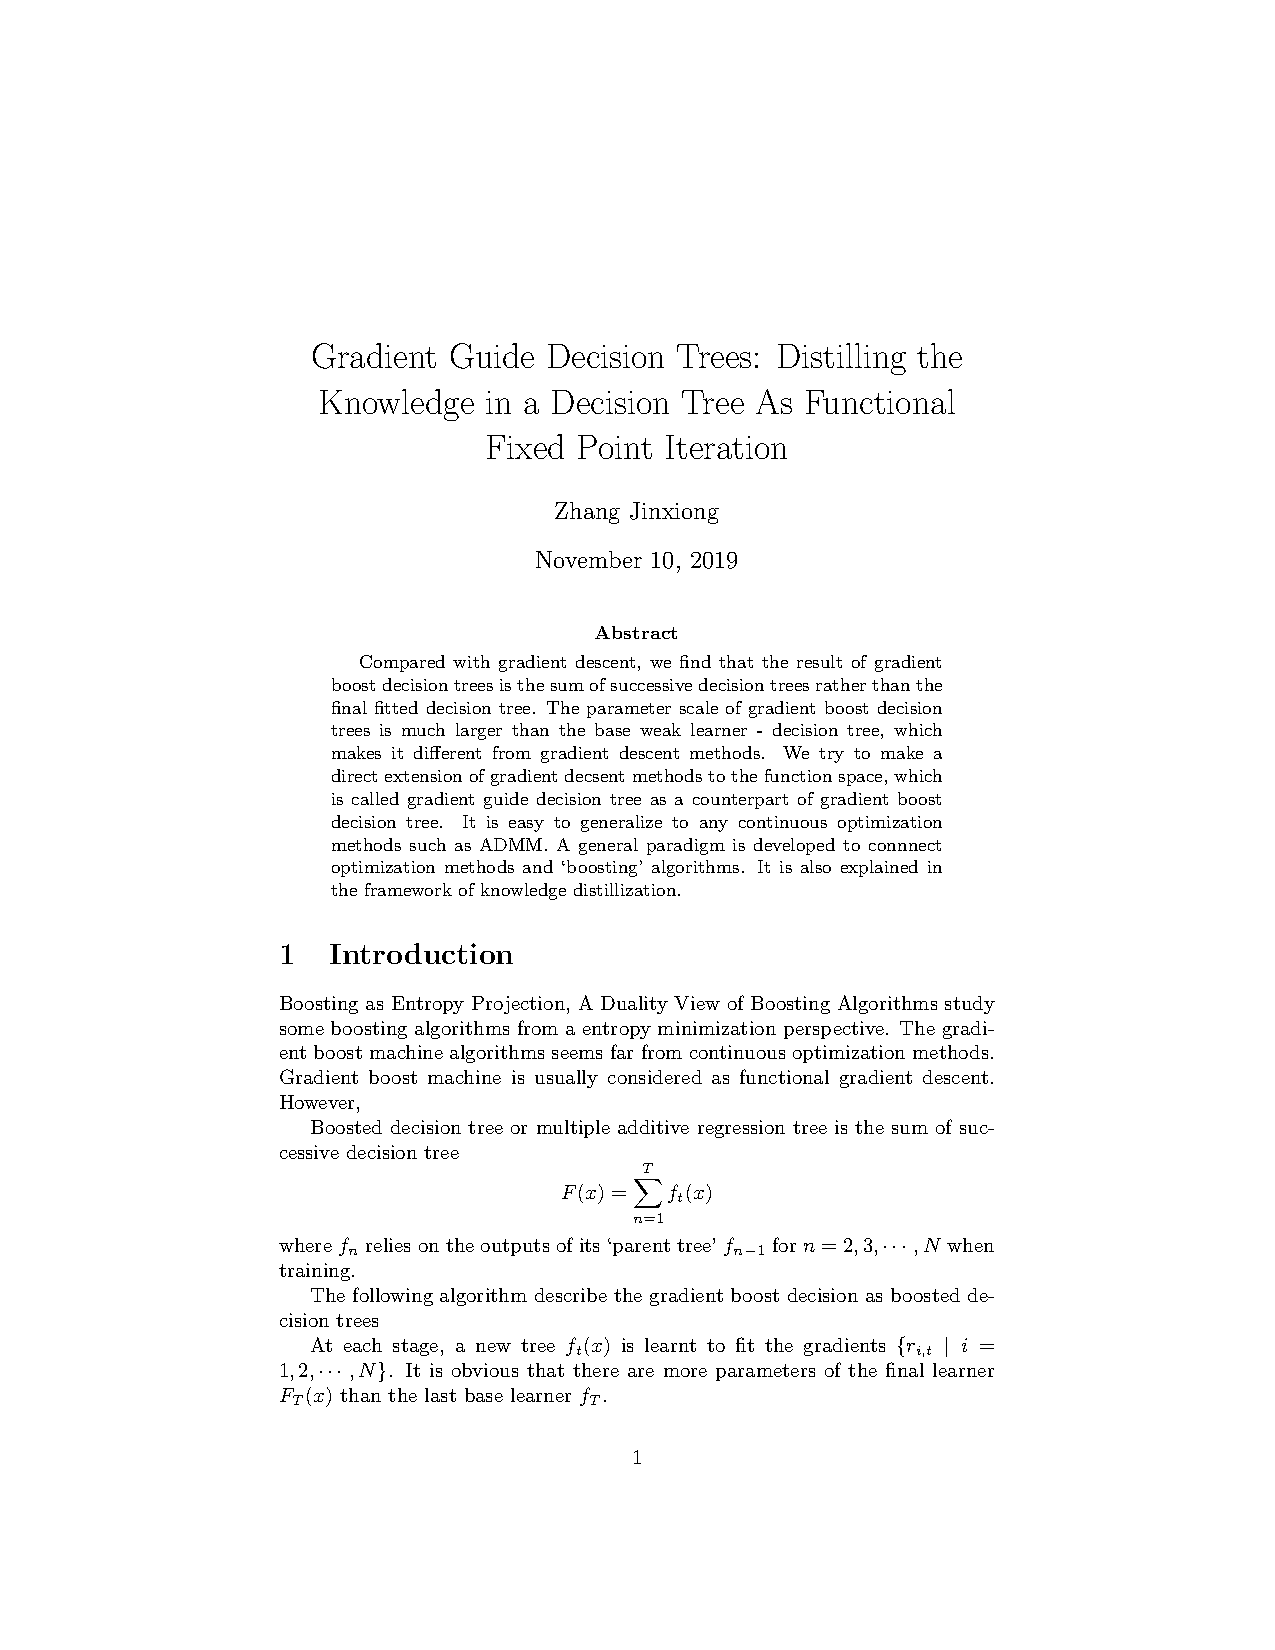
\includegraphics[scale=0.5]{GGDT.png}
%More experiments

\section{Conclusion}

We show the panorama of optimziation and boosting.

\bibliographystyle{plain}
\bibliography{Universal Boost}
\end{document}
